\chapter{Validierung}\label{sec:chapter7}

In diesem Kapitel werden die Ergbnisse des Vergleichs der ConDec - und BPMN-Modelle aus Kapitel 6 mit Hilfe einer Studie validiert.

\section{Forschungsfragen}

\textbf{Forschungsfrage 1a}: 

Ist die Punktsumme bei den Verständnisfragen insgesamt bei BPMN oder bei ConDec höher?\newline



\textbf{Forschungsfrage 1b}: 

Ist die Punktsumme bei den Verständnisfragen bei den kleinen Modellen bei BPMN oder bei ConDec höher?\newline

\textbf{Forschungsfrage 1c}: 

Ist die Punktsumme bei den Verständnisfragen bei den großen Modellen bei BPMN oder bei ConDec höher? \newline

\textbf{Forschungsfrage 1d}: 

Gibt es Unterschiede im Ergebnis in Abhängigkeit des Hintergrundwissesns der Versuchsobjekte über Prozessmodellierung?  \newline

\textbf{Forschungsfrage 2a}: 

Werden bei den Meinungsfragen insgesamt die Modelle von BPMN oder von ConDec präferiert? \newline

\textbf{Forschungsfrage 2b}: 

Werden bei den Meinungsfragen bei den kleinen Modellen die von BPMN oder von ConDec präferiert?\newline

\textbf{Forschungsfrage 2c}: 

Werden bei den Meinungsfragen bei den großen Modellen die von BPMN oder von ConDec präferiert?\newline

\section{Studie}

\subsubsection{Teilnehmer}

Es wurden 32 Studenten und Doktoranden aus dem Bereich Informatik/Medieninformatik befragt. 12 Teilnehmer waren weiblich und 20 männlich (Abbildung \ref{fig:Geschlechterverteilung}). Die allgemeinen demographischen Daten der Probanden können Abbildung \ref{fig:TabelleAllgemeineDaten} entnommen werden. Diese hatten unterschiedliches Hintergrundwissen zum Thema Prozessmodellierung. Wie Abbildung \ref{fig:VerteilungImperativDeklarative} entnommen werden kann, hatten sieben Studienteilnehmer weder in imperativer noch in deklarativer Modellierung Erfahrung. 18 Probanden hatten nur in imperativer Modellierung Erfahrung, jedoch nicht in deklarativer und sieben weitere Teilnehmer hatten in beiden Modellierungssprachen Erfahrung. Die Versuchsobjekte wurden bewusst nach unterschiedlichem Hintergrundwissen zum Thema Prozessmodellierung ausgewählt, um zu prüfen, inwiefern sich die Ergebnisse bei den Verständnisfragen zwischen Personen mit viel und wenig Hintergrundwissen zum Thema Prozessmodellierung unterscheiden.\newline

\begin{figure}[htp]
\begin{center}
  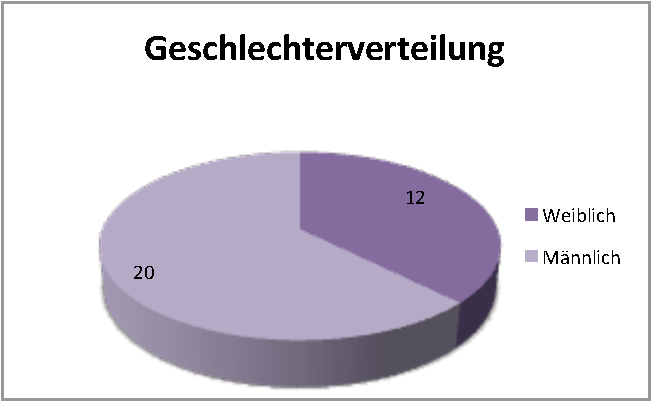
\includegraphics{Geschlechterverteilung} %pdf, jpg, png...
  \caption{Geschlechterverteilung}
  \label{fig:Geschlechterverteilung}
\end{center}
\end{figure}

\begin{figure}[htp]
\begin{center}
  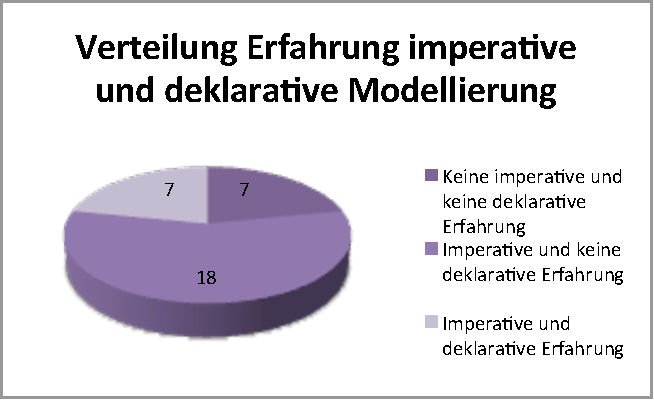
\includegraphics{VerteilungImperativDeklarative} %pdf, jpg, png...
  \caption{Verteilung Erfahrung imperative und deklarative Modellierung}
  \label{fig:VerteilungImperativDeklarative}
\end{center}
\end{figure}

\begin{figure}[htp]
\begin{center}
  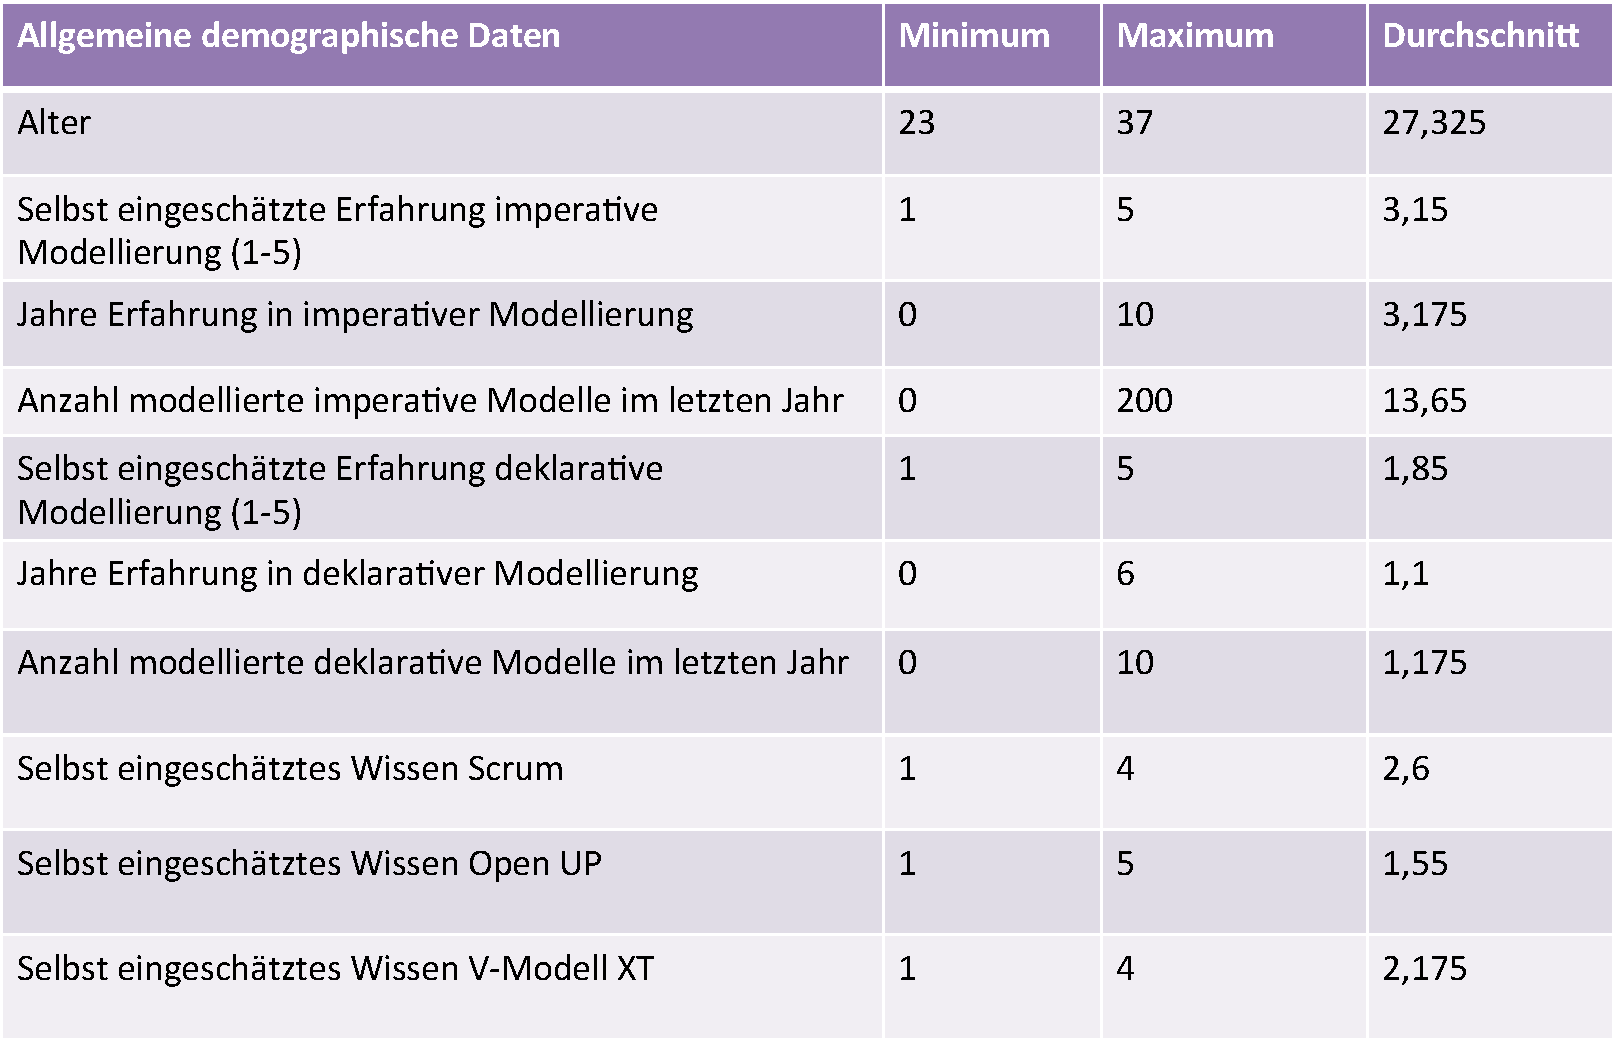
\includegraphics[width=\textwidth]{TabelleAllgemeineDaten} %pdf, jpg, png...
  \caption{Allgemeine demographische Daten}
  \label{fig:TabelleAllgemeineDaten}
\end{center}
\end{figure}









\subsubsection{Design der Studie}
Die Umfrage wurde online mit einem Fragebogen durchgeführt.
In einem ersten Teil